\section{The Electric Potential for Continuous Charge Distributions}
\label{potential_charge_distributions}
\begin{comment}
This lab was written by Matt Trawick in January, 2017.  It incorporates some of the pieces from the original Workshop Physics lab from Dickinson College, but adds some material (potential for a finite rod), and removes some of the introductory stuff, which is now done elsewhere.
\end{comment}

\makelabheader %(Space for student name, etc., defined in master.tex)

\bigskip

\textbf{Introduction} 

You already know how to use the idea of superposition to find the potential due to a handful of point charges.  In this lab, you'll use the same basic idea to find the potential due to a \textit{continuous} distribution of charge, such as a long, uniformly charged rod or a uniformly charged ring.

\bigskip

\textbf{Activity 1: Numerical Approximation of \textit{V} Due to a Charged Rod}

\begin{minipage}{0.64\textwidth}
\begin{quote}
\textbf{Problem:} A thin rod of length $L=20$~cm, with a total positive charge $Q=10$~nC, lies on the $y$ axis between $y=0$ and $y=20$~cm.  Calculate the electric potential $V$ due to the rod at a point $P$ along the $x$ axis a distance $x=15$~cm from the origin. 
\end{quote}

\textbf{Solution:} In this activity, you will estimate $V$ numerically, using Excel.  Divide the rod into ten individual 1~nC pieces, which you can approximate as point charges located at $y=1$~cm, $y=3$~cm, etc., up to $y=19$~cm.  
\end{minipage}
\begin{minipage}{0.35\textwidth}
\vspace{-0.3in}
\raggedleft 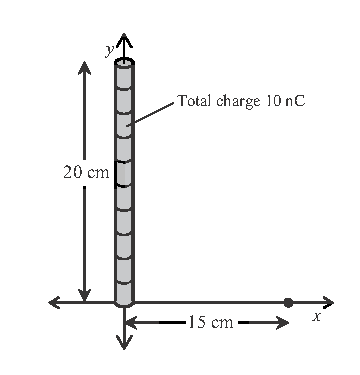
\includegraphics[scale=0.9]{potential_charge_distributions/rod_axes.eps}
\end{minipage}

\begin{enumerate}[labparts]

\item Use Excel to find the electric potential at point $P$ due to \textit{only} the furthest 1~nC point charge, located at $y=19$~cm.  Use $k_e=8.99 \times 10^9$~N$\cdot$m$^2/$C$^2$.  (\textit{Answer:} $\sim 37$ Volts.)
\answerspace{0.5in}

\item Create nine more rows in your Excel table for the other 1~nC charges.  What is the electric potential at point $P$ due to all of them?  (\textit{Answer:} $\sim 494$ Volts, but go ahead and write it to six significant figures.) 
\answerspace{0.5in}

\end{enumerate}

\begin{wrapfigure}[10]{r}{0.30\textwidth}
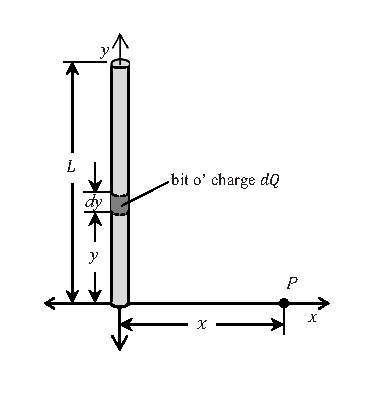
\includegraphics[scale=0.9]{potential_charge_distributions/rod_integral.eps}
\end{wrapfigure}
\textbf{Activity 2: Exact Calculation of \textit{V} Due to a Charged Rod}

Of course, you can imagine making your solution progressively more and more accurate by dividing the rod into smaller and smaller pieces.  And for some very difficult problems, this technique (called ``finite element'' analysis) is the only way to get an answer at all!  But for the thin rod, you can actually calculate an exact solution, by allowing the elements to become infinitely small and performing an integration.

Start by picking a small bit of charge $dQ$ from an arbitrary place in the middle of the rod.  Instead of a discrete sum, you'll integrate
$$V=\int{\frac{k_e\,dQ}{r}}$$
adding up the contributions of each $dQ$ over the whole length of the rod.
\begin{enumerate}[labparts]

\pagebreak[2]
\item Write $dQ$ in terms of $L$, $Q$, and $dy$.
\answerspace{0.3in}

\item Write the distance $r$ from the $dQ$ to the point $P$ in terms the quantities given.  ($y$, $x$, or $L$...) 
\answerspace{0.4in}

\item Now write out the whole integral and solve it.  What are the limits of integration?  One of the integrals given on the right may be useful. \label{part_potential_charge_distributions_exact_rod}
%\answerspace{1.3in}

\begin{minipage}{0.65\textwidth}
\
\end{minipage}
\begin{minipage}{0.34\textwidth}

%\begin{raggedleft}
\textit{World's fourth smallest integral table:}
\begin{align*}
&\int \! \frac{1}{\left (u^2 + a^2 \right )^\frac{3}{2}} \, du=\frac{u}{a^2 \sqrt{u^2 + a^2}} \\
&\int \! \frac{u}{\left (u^2 + a^2 \right )^\frac{3}{2}} \, du=\frac{-1}{\sqrt{u^2 + a^2}} \\
&\int \! \frac{1}{u^2 + a^2} \, du=\frac{1}{a} \tan^{-1} \frac{u}{a} \\
&\int \! \frac{1}{\left (u^2 + a^2 \right )^\frac{1}{2}} \, du=\ln \left | u + \sqrt{u^2 + a^2} \right| \\
\end{align*}
%\end{raggedleft}
\end{minipage}
\item Calculate a precise numerical answer for your result in part \ref{part_potential_charge_distributions_exact_rod} using the same values given in Activity 1.  Your answer should be about the same as what you found in Activity 1.  Which one is more exact?
\answerspace{0.4in}

\end{enumerate}

\textbf{Activity 3: Numerical Approximation of \textit{V} Due to a Charged Ring}\footnote{Activities 3, 4, and 5 are based on previous work (1990-93) by the Department of Physics and Astronomy, Dickinson College. Supported by FIPSE (U.S. Dept. of Ed.) and NSF. Portions of this material were modified locally and have not been classroom tested at Dickinson College.}

\begin{minipage}{0.65\textwidth}
Let's take a look at another example problem, which we'll actually solve three different ways over the next three activities.  

\begin{quote}
\textbf{Problem:} A thin, uniformly charged ring of radius $a=30$~cm has a total charge of $Q = 20\ \mu$C ($20
\times 10^{-6}$~C). Find the electric potential $V$ at a point $P$ a distance $x = 20$~cm from the ring along an axis perpendicular to the ring, passing through its center.
\end{quote}

\textbf{Solution:} As in Activity 1, we will first estimate $V$ numerically, dividing the ring into 20 elements, each of charge $\Delta q = 1\ \mu$C.

\end{minipage}
\begin{minipage}{0.34\textwidth}
\vspace{-0.3in}
\raggedleft 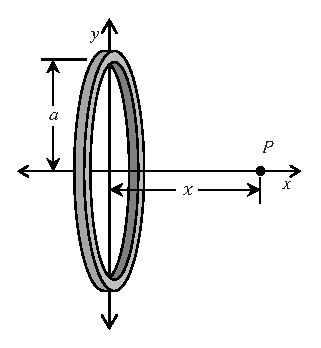
\includegraphics[scale=0.9]{potential_charge_distributions/ring_integral.eps}
\end{minipage}

\begin{enumerate}[labparts]

\item Find $V$ at the point $P$ due to \textit{just one} of the 20 elements.
\answerspace{0.4in}

\item Find $V$ at  point $P$ due to \textit{all} of the 20 elements combined.  You can either use Excel or calculate it by hand; in either case, summarize your procedure below.
\answerspace{0.7in}

\end{enumerate}

\pagebreak[2]
\textbf{Activity 4: Calculating \textit{V} Due to a Charged Ring Using an Integral}

Perhaps you found that your numerical calculation in the last part was fairly trivial---great!  Just for fun, let's see how the integral method for finding $V$ works in this case, and whether we get a more exact answer.

\begin{enumerate}[labparts]

\item Consider a small charge $dQ$ somewhere on the ring, referring back to the figure on the previous page.  Write the integral  
%$V=\int{({k_e/r})\,dQ}$
$\displaystyle V=\int{\frac{k_e\,dQ}{r}}$
with $r$ expressed in terms of quantities given in the figure.
\answerspace{0.6in}

\item The integral you've just written looks hard at first.  But think carefully about what's \textit{constant} in the integral you just wrote.  (What values would be unchanged for the next $dQ$ you choose?)  Rewrite your expression above, pulling any constants outside of the integral sign.
\answerspace{0.5in}

\item What you're left with should be a trivial integral.  Go ahead and solve it, computing a numerical answer for $V$ at $x = 20$~cm.
\answerspace{0.7in}


\item How does your answer above compare to your result in Activity 3?
\answerspace{0.3in}
\end{enumerate}

\textbf{Activity 5: Calculating \textit{V} for the Ring From the Electric Field}

\bigskip

\begin{minipage}{0.60\textwidth}
So far you've found the electric potential for charge distributions using 
%$V=\int{({k_e/r})\,dQ}$
$\displaystyle V=\int{\frac{k_e\,dQ}{r}}$.  
But you also know that 
%$V$ is related to the electric field by 
%$V=-\int{\vv{E} \cdot \vv{ds}}$.  
$\displaystyle V=-\int{\vv{E} \cdot \vv{ds}}$.  
In this activity, we'll find $V$ for the ring a new way: by calculating $\vv{E}$ first, and then getting $V$ from there.

\begin{enumerate}[labparts]

\item What is the direction of $\vv{E}$ at point $P$ due to the \textit{whole} ring?
\answerspace{0.3in}

\item Referring to the figure to the right, write an expression for the magnitude $| \vv{dE} |$ of the electric field due to just a single bit of charge $dQ$.

\end{enumerate}
\end{minipage}
\begin{minipage}{0.39\textwidth}
\vspace{-0.3in}
\raggedleft 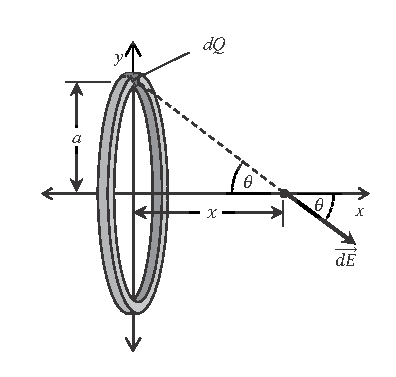
\includegraphics[scale=1.0]{potential_charge_distributions/ring_E_field.eps}
\end{minipage}
$$| \vv{dE}|=\hspace{0.7in}$$
\answerspace{0.1in}

\begin{enumerate}[labparts, start=3] %Without the start=3, it numbers this as (e).  I don't know why.

\item When you add up all of the $\vv{dE}$ from each $dQ$, the $y$ and $z$ components all cancel, leaving only $dE_x$.   What is the magnitude of $dE_x$?  (It should be similar to your answer above, but multiplied by either $\sin \theta$ or $\cos \theta$.)

$$dE_x=\hspace{0.7in}$$
\answerspace{0.1in}

\pagebreak[2]
\item Rewrite the last step, giving  $\sin \theta$ or $\cos \theta$ in terms of a ratio involving $x$, $a$, and/or $\sqrt{x^2 + a^2}$.

$$dE_x=\hspace{0.7in}$$

\medskip

\item Write the complete integral expression for $\vv{E}$.  As in the previous activity, many things inside the integral are actually constant, leaving you with yet another trivial integral to solve.  Solve the integral, and write below a final expression for $\vv{E}$ at an arbitrary point $x$ along the axis.  
\answerspace{0.8in}

\item Now that you have $E$ for every point along the axis, you can integrate it to find $V = - \int{E \, dx}$.  This integral is definitely \textit{not} trivial, but you may find one of the integrals in the table on \pageref{part_potential_charge_distributions_exact_rod} to be helpful.  (Don't forget the integration constant, $+C$.  What will you use for $C$, and why?)
%\answerspace{1.0in}
\vfill

\item Does your answer match with what you found in activities 3 and 4?
\answerspace{0.3in}

\end{enumerate}

\textbf{A General Note About Different Methods For Finding \textit{V}}

In this lab, we used two general methods for finding $V$ from a charge distribution:

\begin{quote}
\textbf{Method 1:} (Activities 1 -- 4) Calculate $V$ directly, using either
$$V = \sum_i{\frac{k_e Q_i}{r_i}}
\qquad  \mathrm{or} \qquad  
V = \int{\frac{k_e \, dQ}{r}}$$
\end{quote}

\begin{quote}
\textbf{Method 2:} (Activity 5) First calculate $\vv{E}$, perhaps using either
$$E = \sum_i{\frac{k_e Q_i}{r^2}}
\qquad  \mathrm{or} \qquad 
\vv{E} = \int{\frac{k_e \, dQ}{r^2}\hat{r}}$$
\phantom{\textbf{Method 2:} }Then find $V$ from $\vv{E}$ using
$$V = - \int{\vv{E} \cdot \vv{ds}}$$
\end{quote}

Both work!  But it should be clear just from the descriptions above that method 2 is going to be a much bigger pain in the badonkadonk most of the time.  (For one thing, method 2 requires two integrals instead of one, and it also requires finding the \textit{vector} $\vv{E}$, which means you have to deal with multiple components.)  Method 1 is almost always your best choice.  The only exception when you might choose method 2 is if you already know $\vv{E}$ or can calculate it relatively easily, for instance by using Gauss' law.


